% Options for packages loaded elsewhere
\PassOptionsToPackage{unicode}{hyperref}
\PassOptionsToPackage{hyphens}{url}
\PassOptionsToPackage{dvipsnames,svgnames,x11names}{xcolor}
%
\documentclass[
]{report}

\usepackage{amsmath,amssymb}
\usepackage{iftex}
\ifPDFTeX
  \usepackage[T1]{fontenc}
  \usepackage[utf8]{inputenc}
  \usepackage{textcomp} % provide euro and other symbols
\else % if luatex or xetex
  \usepackage{unicode-math}
  \defaultfontfeatures{Scale=MatchLowercase}
  \defaultfontfeatures[\rmfamily]{Ligatures=TeX,Scale=1}
\fi
\usepackage{lmodern}
\ifPDFTeX\else  
    % xetex/luatex font selection
\fi
% Use upquote if available, for straight quotes in verbatim environments
\IfFileExists{upquote.sty}{\usepackage{upquote}}{}
\IfFileExists{microtype.sty}{% use microtype if available
  \usepackage[]{microtype}
  \UseMicrotypeSet[protrusion]{basicmath} % disable protrusion for tt fonts
}{}
\makeatletter
\@ifundefined{KOMAClassName}{% if non-KOMA class
  \IfFileExists{parskip.sty}{%
    \usepackage{parskip}
  }{% else
    \setlength{\parindent}{0pt}
    \setlength{\parskip}{6pt plus 2pt minus 1pt}}
}{% if KOMA class
  \KOMAoptions{parskip=half}}
\makeatother
\usepackage{xcolor}
\usepackage[left=20.0mm,right=20.0mm,marginparsep=7.7mm,marginparwidth=70.3mm,top=20mm]{geometry}
\setlength{\emergencystretch}{3em} % prevent overfull lines
\setcounter{secnumdepth}{5}
% Make \paragraph and \subparagraph free-standing
\makeatletter
\ifx\paragraph\undefined\else
  \let\oldparagraph\paragraph
  \renewcommand{\paragraph}{
    \@ifstar
      \xxxParagraphStar
      \xxxParagraphNoStar
  }
  \newcommand{\xxxParagraphStar}[1]{\oldparagraph*{#1}\mbox{}}
  \newcommand{\xxxParagraphNoStar}[1]{\oldparagraph{#1}\mbox{}}
\fi
\ifx\subparagraph\undefined\else
  \let\oldsubparagraph\subparagraph
  \renewcommand{\subparagraph}{
    \@ifstar
      \xxxSubParagraphStar
      \xxxSubParagraphNoStar
  }
  \newcommand{\xxxSubParagraphStar}[1]{\oldsubparagraph*{#1}\mbox{}}
  \newcommand{\xxxSubParagraphNoStar}[1]{\oldsubparagraph{#1}\mbox{}}
\fi
\makeatother

\usepackage{color}
\usepackage{fancyvrb}
\newcommand{\VerbBar}{|}
\newcommand{\VERB}{\Verb[commandchars=\\\{\}]}
\DefineVerbatimEnvironment{Highlighting}{Verbatim}{commandchars=\\\{\}}
% Add ',fontsize=\small' for more characters per line
\usepackage{framed}
\definecolor{shadecolor}{RGB}{241,243,245}
\newenvironment{Shaded}{\begin{snugshade}}{\end{snugshade}}
\newcommand{\AlertTok}[1]{\textcolor[rgb]{0.68,0.00,0.00}{#1}}
\newcommand{\AnnotationTok}[1]{\textcolor[rgb]{0.37,0.37,0.37}{#1}}
\newcommand{\AttributeTok}[1]{\textcolor[rgb]{0.40,0.45,0.13}{#1}}
\newcommand{\BaseNTok}[1]{\textcolor[rgb]{0.68,0.00,0.00}{#1}}
\newcommand{\BuiltInTok}[1]{\textcolor[rgb]{0.00,0.23,0.31}{#1}}
\newcommand{\CharTok}[1]{\textcolor[rgb]{0.13,0.47,0.30}{#1}}
\newcommand{\CommentTok}[1]{\textcolor[rgb]{0.37,0.37,0.37}{#1}}
\newcommand{\CommentVarTok}[1]{\textcolor[rgb]{0.37,0.37,0.37}{\textit{#1}}}
\newcommand{\ConstantTok}[1]{\textcolor[rgb]{0.56,0.35,0.01}{#1}}
\newcommand{\ControlFlowTok}[1]{\textcolor[rgb]{0.00,0.23,0.31}{\textbf{#1}}}
\newcommand{\DataTypeTok}[1]{\textcolor[rgb]{0.68,0.00,0.00}{#1}}
\newcommand{\DecValTok}[1]{\textcolor[rgb]{0.68,0.00,0.00}{#1}}
\newcommand{\DocumentationTok}[1]{\textcolor[rgb]{0.37,0.37,0.37}{\textit{#1}}}
\newcommand{\ErrorTok}[1]{\textcolor[rgb]{0.68,0.00,0.00}{#1}}
\newcommand{\ExtensionTok}[1]{\textcolor[rgb]{0.00,0.23,0.31}{#1}}
\newcommand{\FloatTok}[1]{\textcolor[rgb]{0.68,0.00,0.00}{#1}}
\newcommand{\FunctionTok}[1]{\textcolor[rgb]{0.28,0.35,0.67}{#1}}
\newcommand{\ImportTok}[1]{\textcolor[rgb]{0.00,0.46,0.62}{#1}}
\newcommand{\InformationTok}[1]{\textcolor[rgb]{0.37,0.37,0.37}{#1}}
\newcommand{\KeywordTok}[1]{\textcolor[rgb]{0.00,0.23,0.31}{\textbf{#1}}}
\newcommand{\NormalTok}[1]{\textcolor[rgb]{0.00,0.23,0.31}{#1}}
\newcommand{\OperatorTok}[1]{\textcolor[rgb]{0.37,0.37,0.37}{#1}}
\newcommand{\OtherTok}[1]{\textcolor[rgb]{0.00,0.23,0.31}{#1}}
\newcommand{\PreprocessorTok}[1]{\textcolor[rgb]{0.68,0.00,0.00}{#1}}
\newcommand{\RegionMarkerTok}[1]{\textcolor[rgb]{0.00,0.23,0.31}{#1}}
\newcommand{\SpecialCharTok}[1]{\textcolor[rgb]{0.37,0.37,0.37}{#1}}
\newcommand{\SpecialStringTok}[1]{\textcolor[rgb]{0.13,0.47,0.30}{#1}}
\newcommand{\StringTok}[1]{\textcolor[rgb]{0.13,0.47,0.30}{#1}}
\newcommand{\VariableTok}[1]{\textcolor[rgb]{0.07,0.07,0.07}{#1}}
\newcommand{\VerbatimStringTok}[1]{\textcolor[rgb]{0.13,0.47,0.30}{#1}}
\newcommand{\WarningTok}[1]{\textcolor[rgb]{0.37,0.37,0.37}{\textit{#1}}}

\providecommand{\tightlist}{%
  \setlength{\itemsep}{0pt}\setlength{\parskip}{0pt}}\usepackage{longtable,booktabs,array}
\usepackage{calc} % for calculating minipage widths
% Correct order of tables after \paragraph or \subparagraph
\usepackage{etoolbox}
\makeatletter
\patchcmd\longtable{\par}{\if@noskipsec\mbox{}\fi\par}{}{}
\makeatother
% Allow footnotes in longtable head/foot
\IfFileExists{footnotehyper.sty}{\usepackage{footnotehyper}}{\usepackage{footnote}}
\makesavenoteenv{longtable}
\usepackage{graphicx}
\makeatletter
\newsavebox\pandoc@box
\newcommand*\pandocbounded[1]{% scales image to fit in text height/width
  \sbox\pandoc@box{#1}%
  \Gscale@div\@tempa{\textheight}{\dimexpr\ht\pandoc@box+\dp\pandoc@box\relax}%
  \Gscale@div\@tempb{\linewidth}{\wd\pandoc@box}%
  \ifdim\@tempb\p@<\@tempa\p@\let\@tempa\@tempb\fi% select the smaller of both
  \ifdim\@tempa\p@<\p@\scalebox{\@tempa}{\usebox\pandoc@box}%
  \else\usebox{\pandoc@box}%
  \fi%
}
% Set default figure placement to htbp
\def\fps@figure{htbp}
\makeatother

\usepackage{unicode-math}
\DeclareMathOperator{\var}{\mathbb{V}\mathrm{ar}}
\DeclareMathOperator{\cov}{\mathbb{C}\mathrm{ov}}
\newcommand\eqc{\stackrel{c}{=}}
\newcommand{\bv}[1]{\symbfit{#1}}
\setmainfont{XITS}
\setmathfont{XITS Math}


\usepackage{tcolorbox}
\tcbuselibrary{most}


% Define styles for theorem, lemma, proof, etc.
\newtcolorbox{mytheorem}[1][]{colback=blue!5!white, colframe=blue!75!black,
fonttitle=\bfseries, title=Theorem, #1}

\newtcolorbox{mylemma}[1][]{colback=green!5!white, colframe=green!75!black,
fonttitle=\bfseries, title=Lemma, #1}

\newtcolorbox{myproof}[1][]{colback=red!5!white, colframe=red!75!black,
fonttitle=\bfseries, title=Proof, #1}

\newtcolorbox{myexample}[1][]{colback=yellow!5!white, colframe=yellow!75!black,
fonttitle=\bfseries, title=Example, #1}
\makeatletter
\@ifpackageloaded{caption}{}{\usepackage{caption}}
\AtBeginDocument{%
\ifdefined\contentsname
  \renewcommand*\contentsname{Table of contents}
\else
  \newcommand\contentsname{Table of contents}
\fi
\ifdefined\listfigurename
  \renewcommand*\listfigurename{List of Figures}
\else
  \newcommand\listfigurename{List of Figures}
\fi
\ifdefined\listtablename
  \renewcommand*\listtablename{List of Tables}
\else
  \newcommand\listtablename{List of Tables}
\fi
\ifdefined\figurename
  \renewcommand*\figurename{Figure}
\else
  \newcommand\figurename{Figure}
\fi
\ifdefined\tablename
  \renewcommand*\tablename{Table}
\else
  \newcommand\tablename{Table}
\fi
}
\@ifpackageloaded{float}{}{\usepackage{float}}
\floatstyle{ruled}
\@ifundefined{c@chapter}{\newfloat{codelisting}{h}{lop}}{\newfloat{codelisting}{h}{lop}[chapter]}
\floatname{codelisting}{Listing}
\newcommand*\listoflistings{\listof{codelisting}{List of Listings}}
\makeatother
\makeatletter
\makeatother
\makeatletter
\@ifpackageloaded{caption}{}{\usepackage{caption}}
\@ifpackageloaded{subcaption}{}{\usepackage{subcaption}}
\makeatother
\makeatletter
\@ifpackageloaded{tcolorbox}{}{\usepackage[skins,breakable]{tcolorbox}}
\makeatother
\makeatletter
\@ifundefined{shadecolor}{\definecolor{shadecolor}{rgb}{.97, .97, .97}}{}
\makeatother
\makeatletter
\@ifundefined{codebgcolor}{\definecolor{codebgcolor}{HTML}{EEEEEE}}{}
\makeatother
\makeatletter
\ifdefined\Shaded\renewenvironment{Shaded}{\begin{tcolorbox}[frame hidden, sharp corners, enhanced, boxrule=0pt, breakable, colback={codebgcolor}]}{\end{tcolorbox}}\fi
\makeatother

\usepackage{bookmark}

\IfFileExists{xurl.sty}{\usepackage{xurl}}{} % add URL line breaks if available
\urlstyle{same} % disable monospaced font for URLs
\hypersetup{
  pdftitle={Efficient Filtering and Fitting of Models Derived from Integro-Difference Equations},
  pdfauthor={Evan Tate Paterson Hughes},
  colorlinks=true,
  linkcolor={blue},
  filecolor={Maroon},
  citecolor={Blue},
  urlcolor={Blue},
  pdfcreator={LaTeX via pandoc}}


\title{Efficient Filtering and Fitting of Models Derived from
Integro-Difference Equations}
\author{Evan Tate Paterson Hughes}
\date{}

\begin{document}
\maketitle

\renewcommand*\contentsname{Table of contents}
{
\hypersetup{linkcolor=}
\setcounter{tocdepth}{2}
\tableofcontents
}

\chapter{\texorpdfstring{Fitting IDEM using
\texttt{jax\_idem}}{Fitting IDEM using jax\_idem}}\label{fitting-idem-using-jax_idem}

The primary use of the jax\_idem package is to fit Integro-difference
equation models to data.

Currently, the only supported way to do this is through
maximum-likelihood estimation with the kalman/information filter and
OPTAX.

\section{Simple example; synthetic simple
data}\label{simple-example-synthetic-simple-data}

We will start by simulating from a simple IDEM with only three time
steps. We can quickly make a model using \texttt{gen\_example\_idem};

\begin{Shaded}
\begin{Highlighting}[]
\ImportTok{import}\NormalTok{ sys}
\ImportTok{import}\NormalTok{ os}
\NormalTok{sys.path.append(os.path.abspath(}\StringTok{\textquotesingle{}../src/jax\_idem\textquotesingle{}}\NormalTok{))}

\ImportTok{import}\NormalTok{ jax.random }\ImportTok{as}\NormalTok{ rand}
\ImportTok{import}\NormalTok{ jax.numpy }\ImportTok{as}\NormalTok{ jnp}
\ImportTok{import}\NormalTok{ jax}
\ImportTok{import}\NormalTok{ matplotlib.pyplot }\ImportTok{as}\NormalTok{ plt}
\ImportTok{import}\NormalTok{ filter\_smoother\_functions }\ImportTok{as}\NormalTok{ fsf}
\ImportTok{import}\NormalTok{ plotly.express }\ImportTok{as}\NormalTok{ px}
\ImportTok{import}\NormalTok{ plotly.io }\ImportTok{as}\NormalTok{ pio}
\ImportTok{import}\NormalTok{ plotly.graph\_objs }\ImportTok{as}\NormalTok{ go}
\ImportTok{import}\NormalTok{ pandas }\ImportTok{as}\NormalTok{ pd}

\ImportTok{import}\NormalTok{ utilities}
\ImportTok{import}\NormalTok{ IDEM }\ImportTok{as}\NormalTok{ idem}
\ImportTok{import}\NormalTok{ filter\_smoother\_functions }\ImportTok{as}\NormalTok{ fsf}
\end{Highlighting}
\end{Shaded}

\begin{Shaded}
\begin{Highlighting}[]
\NormalTok{key }\OperatorTok{=}\NormalTok{ jax.random.PRNGKey(}\DecValTok{1}\NormalTok{)}
\NormalTok{keys }\OperatorTok{=}\NormalTok{ rand.split(key, }\DecValTok{3}\NormalTok{)}

\NormalTok{process\_basis }\OperatorTok{=}\NormalTok{ utilities.place\_basis(nres}\OperatorTok{=}\DecValTok{1}\NormalTok{, min\_knot\_num}\OperatorTok{=}\DecValTok{5}\NormalTok{)}
\NormalTok{nbasis }\OperatorTok{=}\NormalTok{ process\_basis.nbasis}

\NormalTok{m\_0 }\OperatorTok{=}\NormalTok{ jnp.zeros(nbasis).at[}\DecValTok{7}\NormalTok{].}\BuiltInTok{set}\NormalTok{(}\DecValTok{1}\NormalTok{)}
\NormalTok{sigma2\_0 }\OperatorTok{=} \FloatTok{0.01}

\NormalTok{truemodel }\OperatorTok{=}\NormalTok{ idem.gen\_example\_idem(}
\NormalTok{    keys[}\DecValTok{0}\NormalTok{], k\_spat\_inv}\OperatorTok{=}\VariableTok{True}\NormalTok{,}
\NormalTok{    process\_basis}\OperatorTok{=}\NormalTok{process\_basis,}
\NormalTok{    m\_0}\OperatorTok{=}\NormalTok{m\_0, sigma2\_0}\OperatorTok{=}\NormalTok{sigma2\_0}
\NormalTok{)}

\CommentTok{\# Simulation}
\NormalTok{T }\OperatorTok{=} \DecValTok{3}
                                            
\NormalTok{process\_data, obs\_data }\OperatorTok{=}\NormalTok{ truemodel.simulate(nobs}\OperatorTok{=}\DecValTok{50}\NormalTok{, T}\OperatorTok{=}\NormalTok{T }\OperatorTok{+} \DecValTok{1}\NormalTok{, key}\OperatorTok{=}\NormalTok{keys[}\DecValTok{1}\NormalTok{])}

\NormalTok{process\_data.show\_plot()}
\end{Highlighting}
\end{Shaded}

\begin{verbatim}
/home/tate/MyProjects/JAX-IDEM/src/jax_idem/utilities.py:393: UserWarning:

Matplotlib is currently using module://matplotlib_inline.backend_inline, which is a non-GUI backend, so cannot show the figure.
\end{verbatim}

\pandocbounded{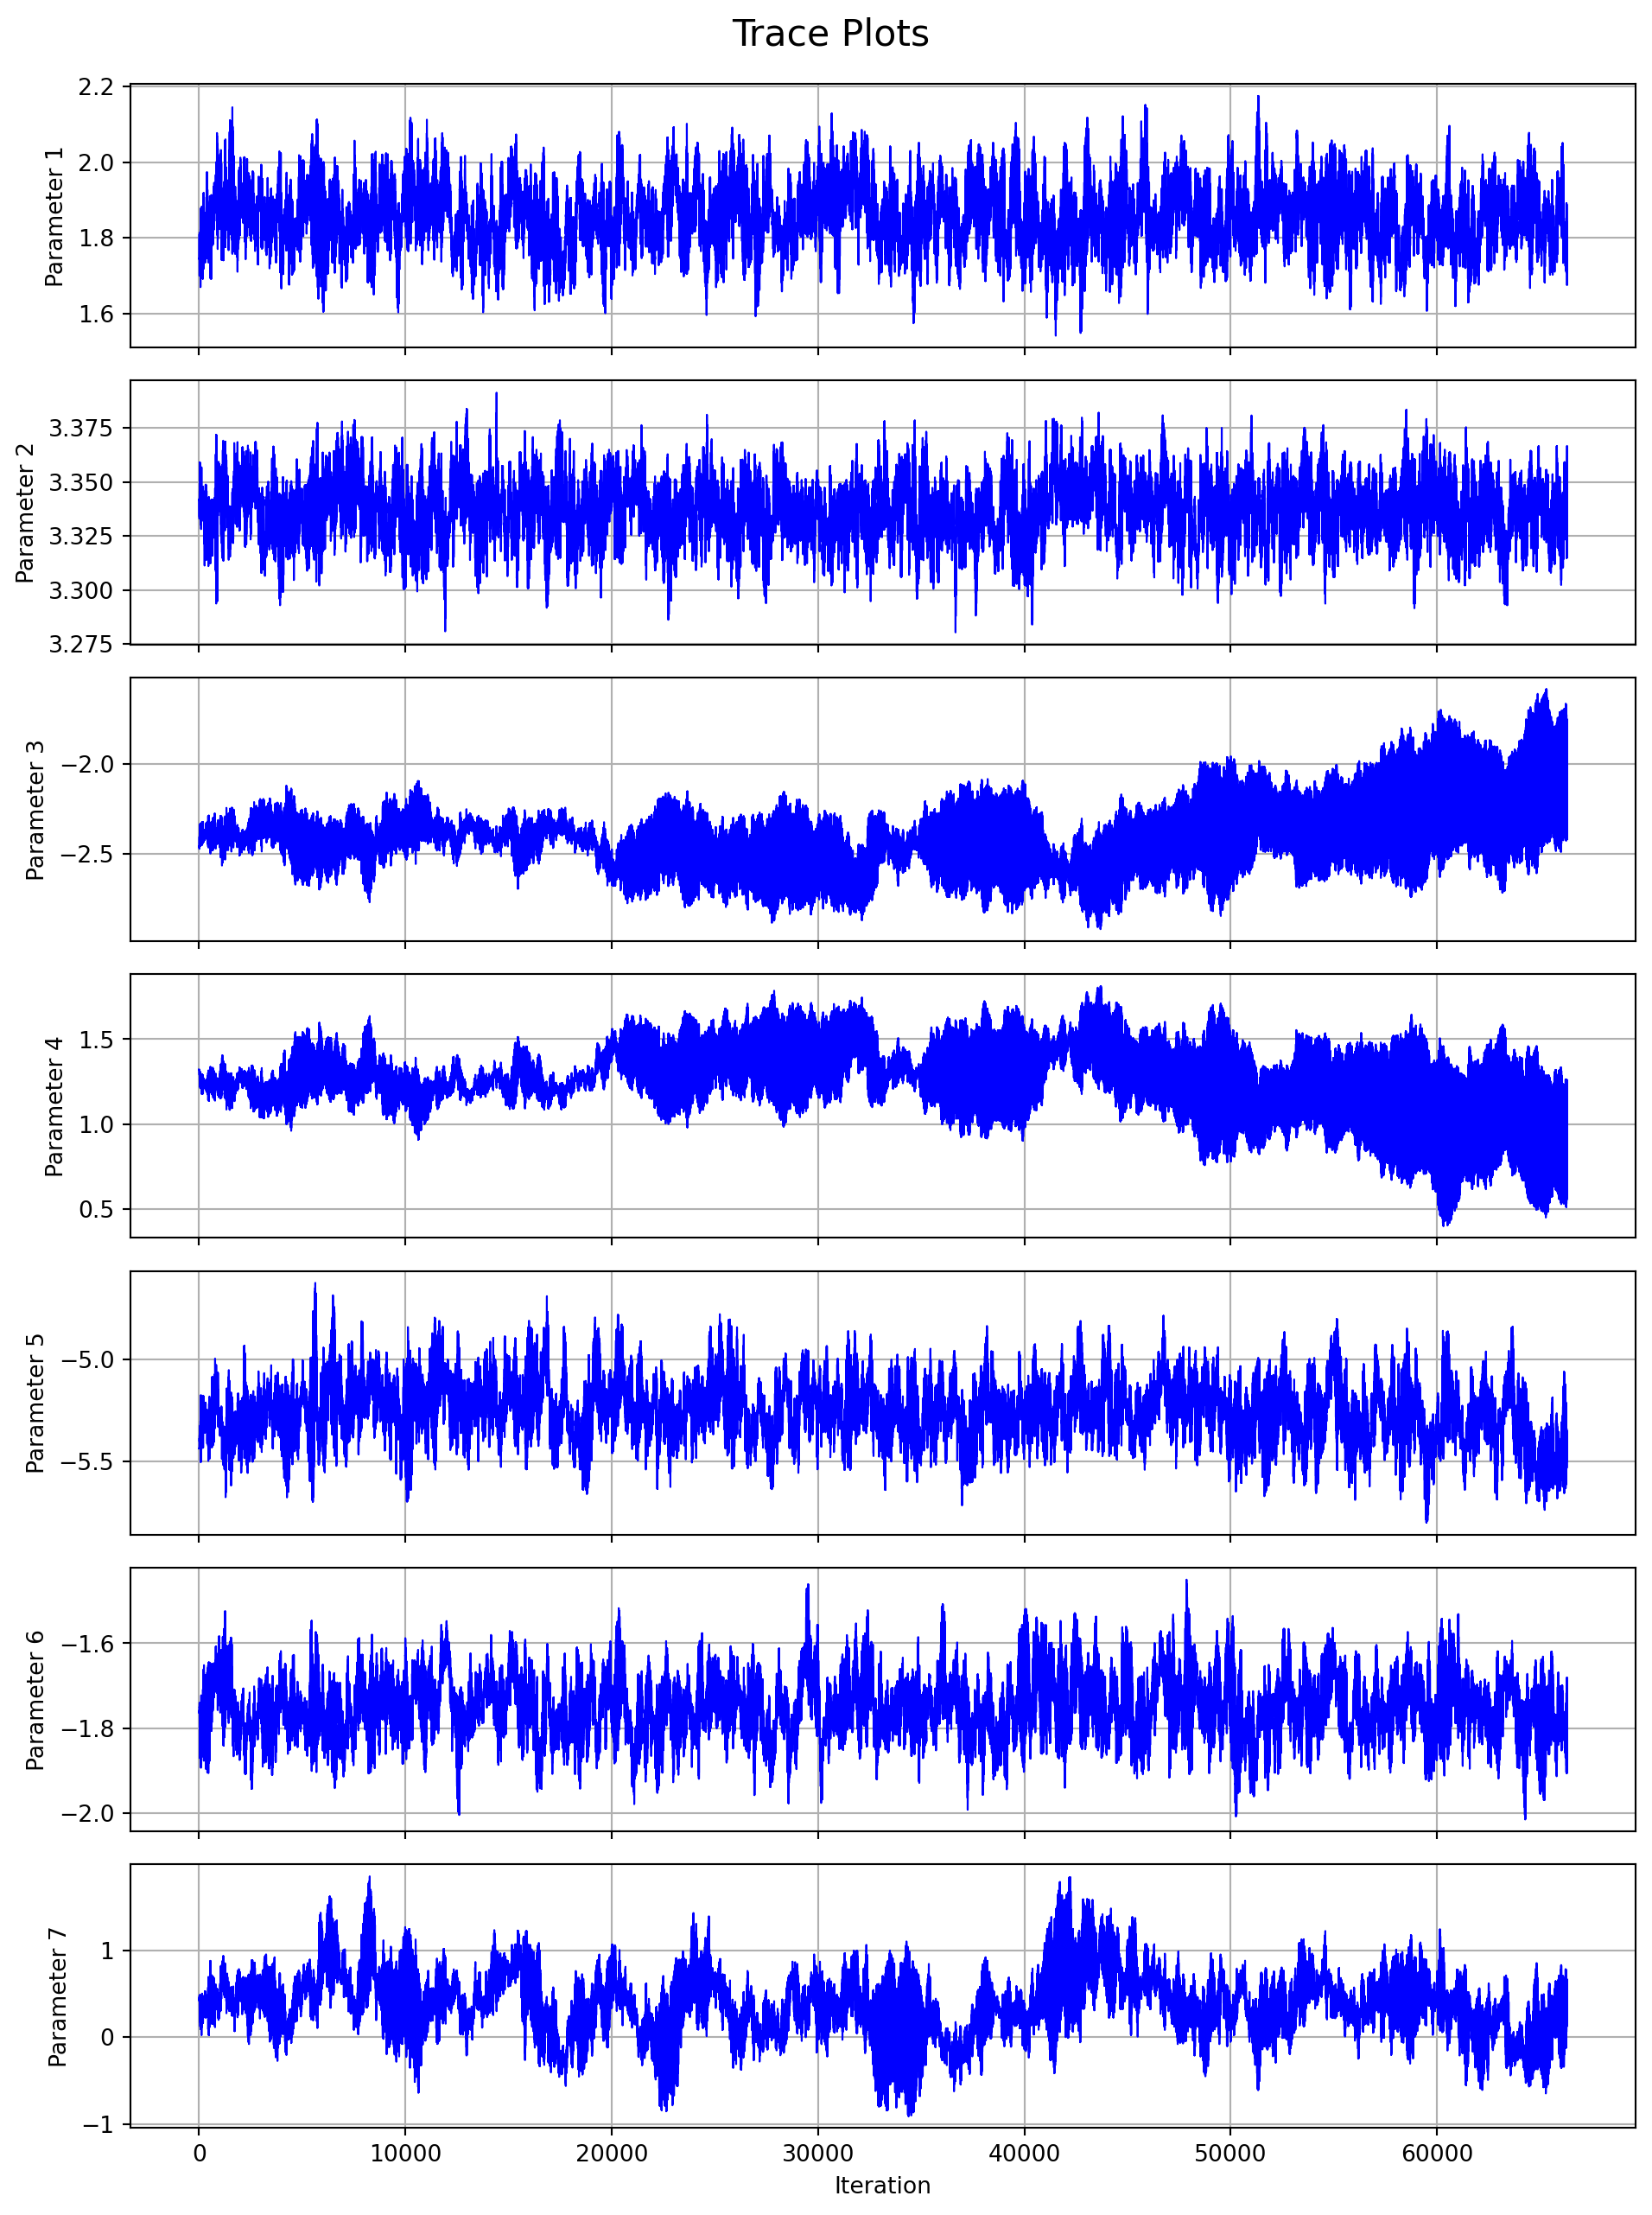
\includegraphics[keepaspectratio]{fit_example_files/figure-pdf/cell-3-output-2.pdf}}




\end{document}
